\documentclass{article}
\usepackage{graphicx} % Required for inserting images
\usepackage{todonotes}
\usepackage[colorlinks=true, allcolors=blue]{hyperref}
\usepackage{biblatex}
\usepackage{multirow}
\usepackage{caption}
\usepackage{subcaption}
\addbibresource{references.bib}

\newcommand\todoJason[1]{\todo[author=Jason,color=yellow,inline]{#1}}
\newcommand\todoMichael[1]{\todo[author=Michael,color=green,inline]{#1}}
\newcommand\todoChris[1]{\todo[author=Chris,color=orange,inline]{#1}}

\title{How Super are Super Computers?}
\author{Jason Stewart\\
\textit{jastewart@unm.edu} 
\and
Michael Servilla\\
\textit{chico@unm.edu}
\and
Christopher Leap\\
\textit{cleap@unm.edu}
\date{\today}
}

\begin{document}

\maketitle

\todo{Finish report writing by Wed Nov 29}
\todoJason{Proofread report and make presentation slides}
\section{Introduction}
General perceptions suggest that the computers in high-performance computing (HPC) centers are faster and more powerful than the commodity computers we use outside of these environments. Beyond considering the network or clustering capabilities of HPC centers, our objective is to evaluate the true extent of these supercomputers' capabilities. We aim to compare the performance of several computers within an HPC center with that of business-grade computers located outside of an HPC center, as well as with commodity computers typically owned by individuals (e.g., laptops and desktop personal computers). We will conduct two types of benchmark tests: one focusing on low-compute network-intensive tasks and the other concentrating on high-compute tasks with minimal reliance on networking. Utilizing these benchmark tests, we will employ `time to completion' as a proxy for performance and compare the results across different computer types.

\section{Methods}

\subsection{Benchmarks}
We created two benchmarks for this project. The first benchmark, \textit{all\_to\_all}, reports the average and standard deviation of the amount of time to takes to run one iteration of MPI\_Alltoall with a message size of 4196 bytes.

The second benchmark, \textit{count\_primes}, reports the average and standard deviation of the amount of time to takes for each process to count prime numbers between 0 and 10000 and perform a single MPI\_Allgather at the end.

We ran the \textit{count\_primes} benchmark using 1, 2, 4, 6, 8, 16, 32, 64, and 128 processes. We ran the \textit{all\_to\_all} benchmark with up to 32 processes. With more processes than 32, the \textit{all\_to\_all} requires too much memory and cannot be run.

The code for these benchmarks is included in our GitHub repository \cite{repo}.

\subsection{Computers}
A total of ten computers were used in our study. These included three HPC computers from the University of New Mexico's Center for Advanced Research Computing (CARC) – Hopper, Wheeler, and Xena; three business-grade computers housed at the University of New Mexico’s computer science department – Trucks, Leda, and Sahu; and four commodity-class computers owned individually, which comprise three laptops (Aureolin, Ocotillo, and Yucca) and one desktop (Celeste). All ten computers contain central processing units manufactured by Intel and varied in specifications such as the number of cores per node, cores per socket, and processing speeds.
\begin{table}[h!]
\centering
\begin{tabular}{|c|c|c|c|c|}
\hline
\textbf{Computer} & \textbf{CPU Model} & \textbf{Cores} & \textbf{Cores} & \textbf{Clock} \\
 & & \textbf{per} & \textbf{per} & \textbf{Rate} \\
 & & \textbf{Node} & \textbf{Socket} & \textbf{(MHz)} \\
\hline
Hopper & Intel(R) Xeon(R) Gold 6226R & 64 & 16 & 2900 \\
Wheeler & Intel(R) Xeon(R) X5550 & 8 & 4 & 2670 \\
Xena & Intel(R) Xeon(R) CPU E5-2640 v3 & 16 & 8 & 2600 \\
Aureolin & Intel(R) Core(TM) i7-12700H & 10 & 10 & 2688 \\
Celeste & Intel(R) Core(TM) i7-8700 & 6 & 6 & 3200 \\
Leda & Intel(R) Core(TM) i9-9900K & 16 & 8 & 3600 \\
Trucks & Intel(R) Xeon(R) CPU E5-2637 v4 & 4 & 1 & 3500 \\
Sahu & Intel(R) Xeon(R) Gold 6338 & 128 & 32 & 2000 \\
Ocotillo & Intel(R) Core(TM) i7-5500U & 4 & 2 & 2400 \\
Yucca & Intel(R) Core(TM) i9-10885H & 16 & 8 & 2400 \\
\hline
\end{tabular}
\caption{Specifications of Computers Used in Study}
\label{table:computers}
\end{table}

\section{Results}

\begin{figure}[h]
    \centering
    \begin{subfigure}[b]{0.49\textwidth}
         \centering
         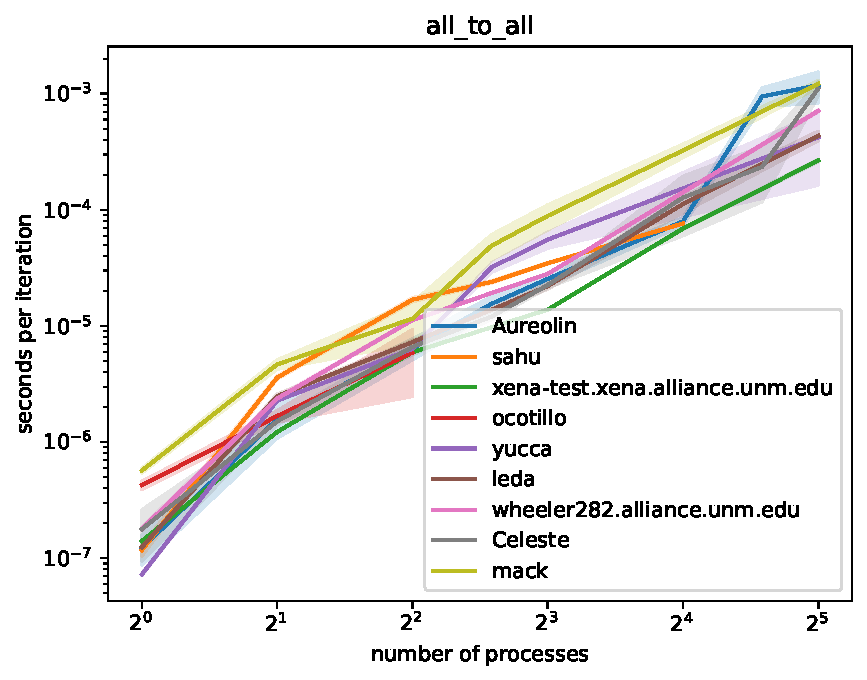
\includegraphics[width=\textwidth]{figures/final/all_to_all.pdf}
         \caption{The results of ``all\_to\_all"}
         \label{fig:all_to_all}
     \end{subfigure}
     \hfill
     \begin{subfigure}[b]{0.49\textwidth}
         \centering
         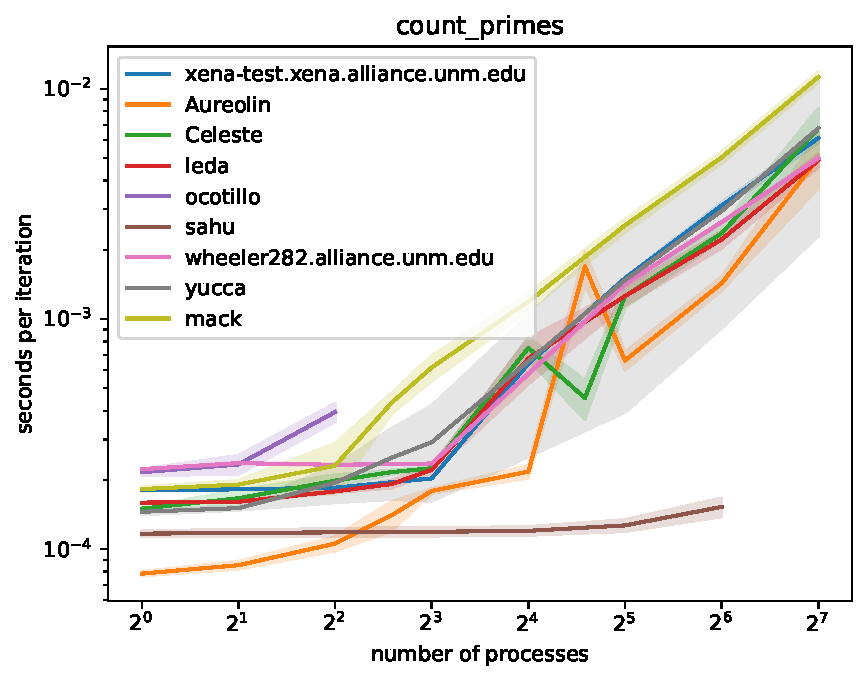
\includegraphics[width=\textwidth]{figures/final/count_primes.pdf}
         \caption{The results of ``count\_primes"}
         \label{fig:count_primes}
     \end{subfigure}
     \hfill
    \caption{The benchmark results across computers. Each line is the mean benchmark time across 800 repetitions with one standard deviation either side of the mean shaded in. The red x's denote we ran using more tasks than the number of CPU cores available. }
    \label{fig:direct}
\end{figure}

We ran the ``all\_to\_all" and ``count\_primes" benchmarks for each of the computers. Each benchmark repeats 1000 times consecutively, which we time and divide by 1000 to get the time for one benchmark iteration. We repeat this process 800 times. For Figure \ref{fig:direct} and Figure \ref{fig:normalized}, each line corresponds to the mean across the 800 runs with the shaded area corresponding to one standard deviation either side of the mean.

Figure \ref{fig:direct} shows the results of the benchmarks using the timings directly. We expected the performance of commodity computers to be better than that of the supercomputers, since supercomputers are optimized for networking performance, while commodity computers are optimized to be used without networking. However, the results in Figure \ref{fig:direct} show that the benchmark results for the supercomputers - hopper, xena, and wheeler, fall in the middle of the benchmark results for the commodity computers. This suggests that being part of a supercomputer has little bearing on the performance for our benchmarks.

\begin{figure}[h!]
    \centering
    \begin{subfigure}[b]{0.49\textwidth}
         \centering
         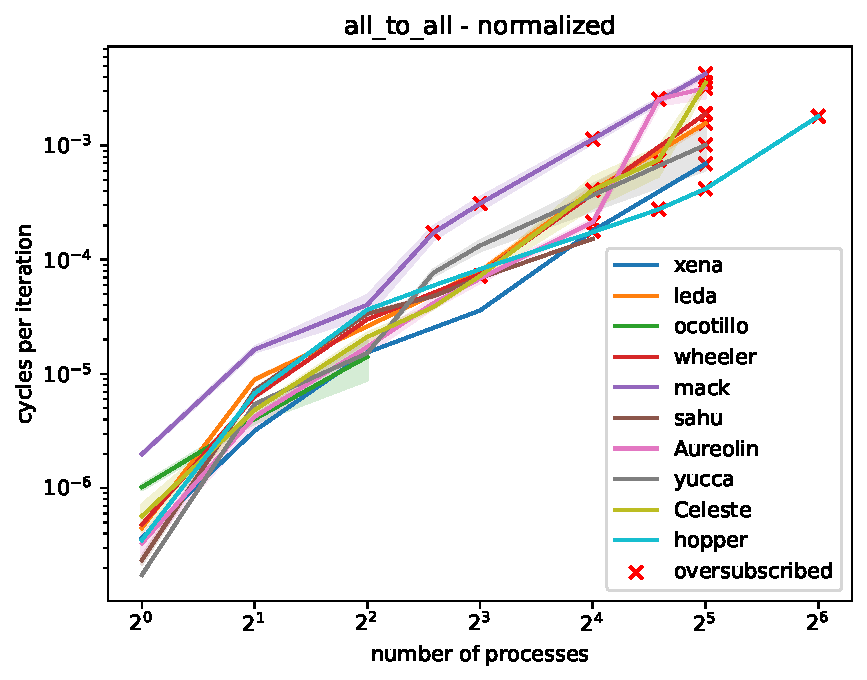
\includegraphics[width=\textwidth]{figures/final/all_to_all_normalized.pdf}
         \caption{The results of ``all\_to\_all"}
         \label{fig:all_to_all}
     \end{subfigure}
     \hfill
     \begin{subfigure}[b]{0.49\textwidth}
         \centering
         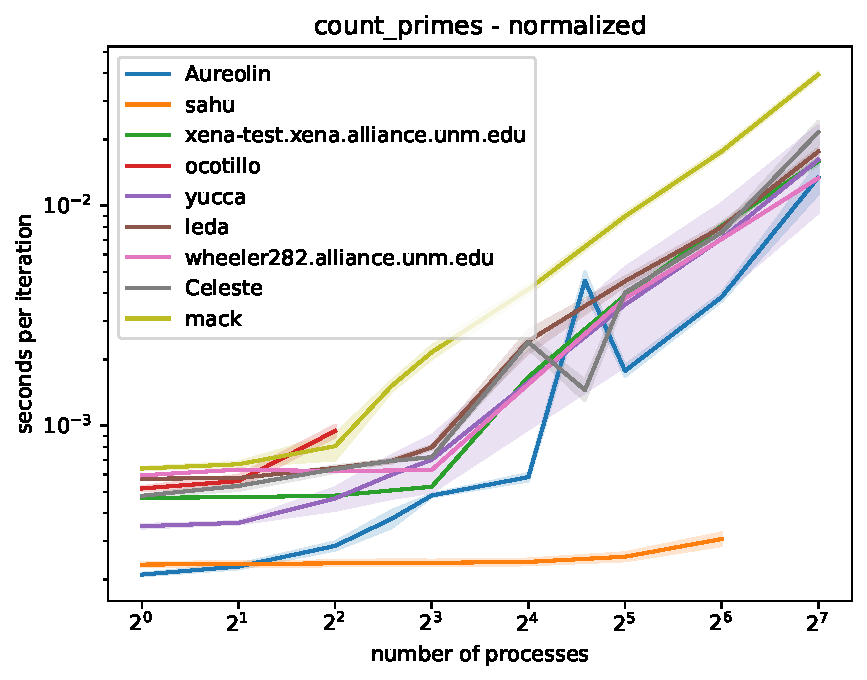
\includegraphics[width=\textwidth]{figures/final/count_primes_normalized.pdf}
         \caption{The results of ``count\_primes"}
         \label{fig:count_primes}
     \end{subfigure}
     \hfill
    \caption{The benchmark results across computers. Each line is the ``normalized" mean benchmark result in cycles per benchmark across 800 repetitions with one standard deviation either side of the mean shaded in. The red x's denote we ran using more tasks than the number of CPU cores available. }
    \label{fig:normalized}
\end{figure}

We then attempt to ``normalize" the results by multiplying each benchmark timing (seconds per benchmark) by the computer's clock speed (cycles per second) to get the timings in cycles per benchmark. We hypothesized that this would exaggerate any differences between the computers that was not due to variations in clock speed. Figure \ref{fig:normalized} shows the results of this experiment. We observe that the ``normalized" performance is nearly identical to the ``un-normalized" performance. This suggests that either clock speed did not play a significant role in the benchmark performance or that our normalization technique does not accurately account for the variations in performance due to clock speed.

\begin{figure}[h]
    \centering
    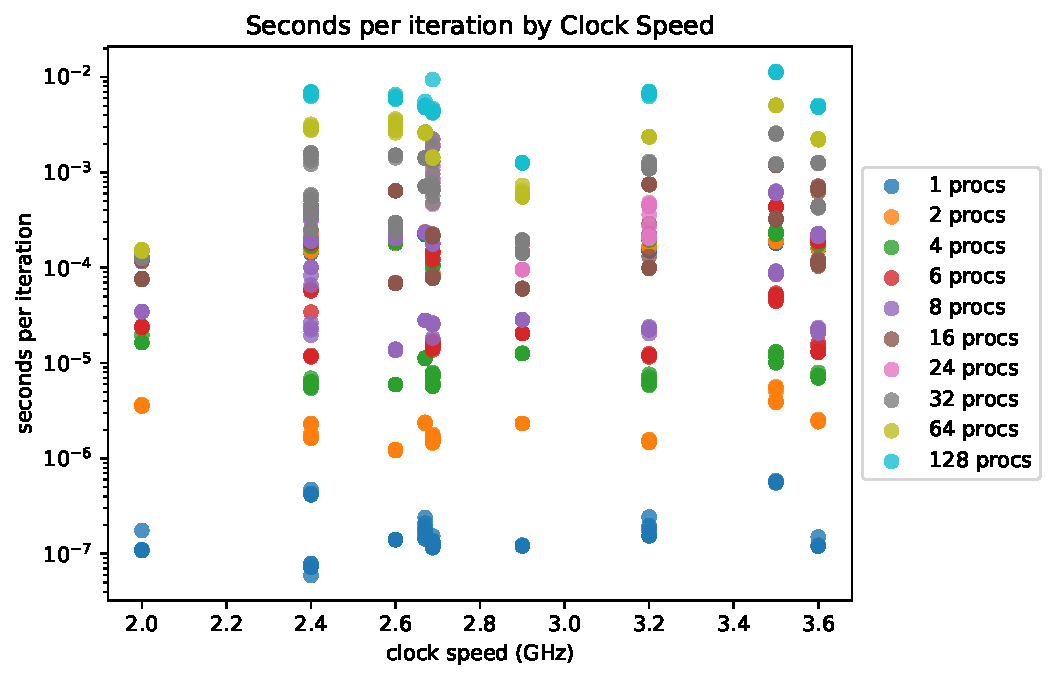
\includegraphics[width=0.6\textwidth]{figures/final/correlation.pdf}
    \caption{A correlation plot, showing the relationship between the clock speed of a cpu and how long each benchmark takes to run across the various sizes of benchmark. }
    \label{fig:correlation}
\end{figure}

To further investigate the role of clock speed in our benchmark performances, we examined the correlation between clock speed and benchmark timings for different scale runs, shown in Figure \ref{fig:correlation}. What we see is for a fixed number of processes, the clock speed has little influence on the benchmark performance. The only notable exception is given by Sahu, with a clock speed of 2.0 GHz. We guess this is because Sahu has 128 CPU cores, so it is better suited to handle the larger-scale benchmarks.

\begin{figure}[h]
    \centering
    \begin{subfigure}[b]{0.49\textwidth}
         \centering
         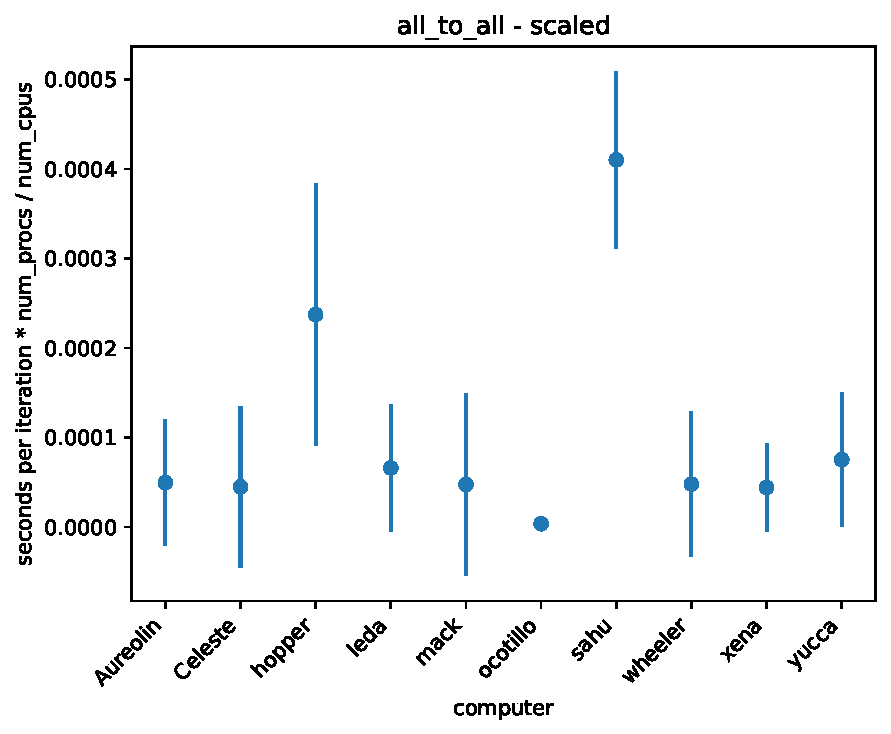
\includegraphics[width=\textwidth]{figures/final/all_to_all_scaled.pdf}
         \caption{The results of ``all\_to\_all"}
         \label{fig:all_to_all}
     \end{subfigure}
     \hfill
     \begin{subfigure}[b]{0.49\textwidth}
         \centering
         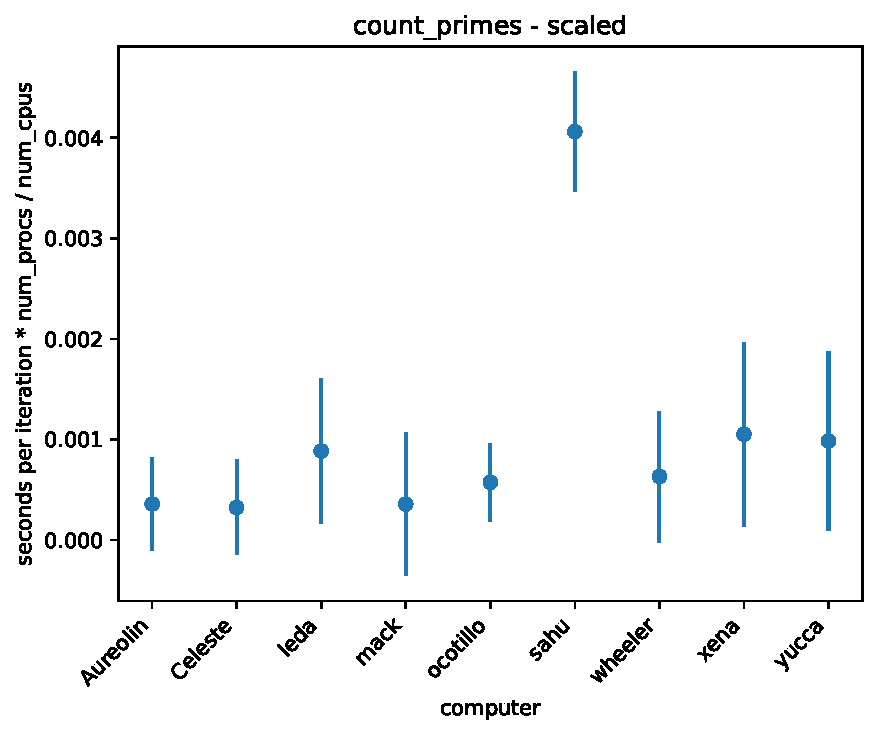
\includegraphics[width=\textwidth]{figures/final/count_primes_scaled.pdf}
         \caption{The results of ``count\_primes"}
         \label{fig:normalized}
     \end{subfigure}
     \hfill
    \caption{The ``scaled" mean benchmark results. }
    \label{fig:scaled}
\end{figure}

Next, we make a ``scaled" comparison between the computers, shown in Figure \ref{fig:scaled}. To do this, we multiply each benchmark time by the number of processes used and divide by the total number of cpu cores on the computer. This gives us a distribution of results for each computer in terms of the percentage of cores used. We see that the supercomputers and commodity computers fall within the same ranges, except for Hopper and Sahu. We believe Sahu and Hopper stand out because they have significantly more cores than the other machines. Sahu has 128 cores and Hopper has 64 cores, while the next highest number of cores is 16.


\begin{figure}[h]
    \centering
    \begin{subfigure}[b]{0.49\textwidth}
         \centering
         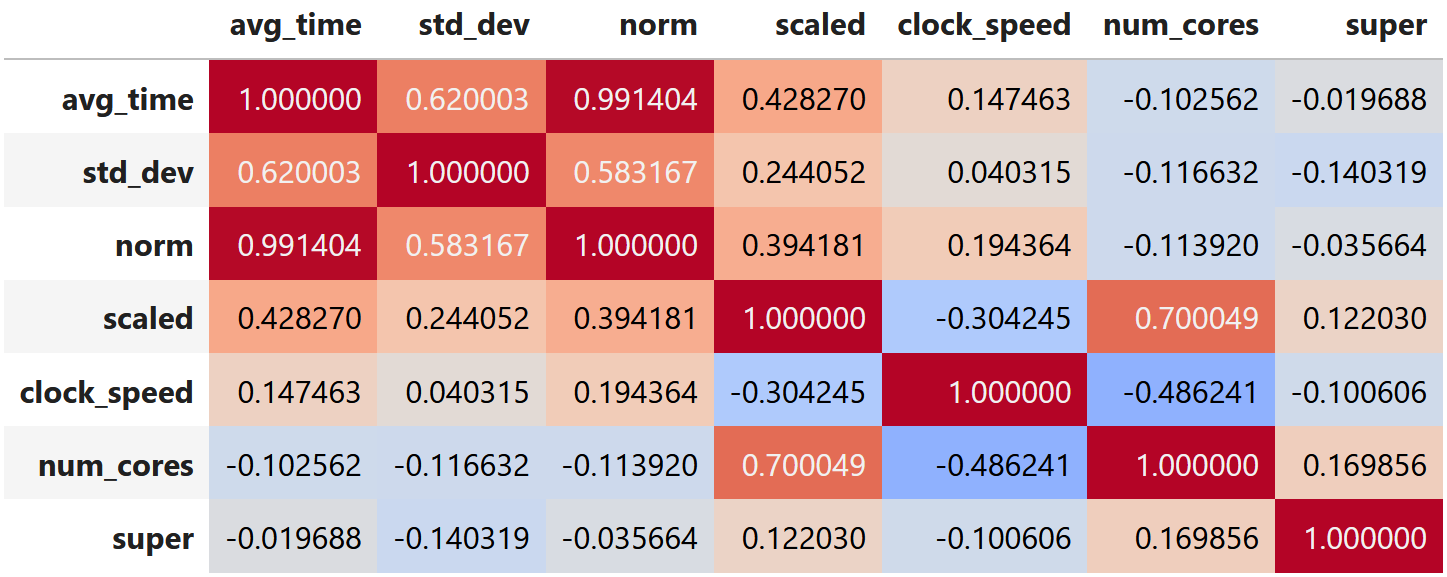
\includegraphics[width=\textwidth]{figures/final/xcorr_all_to_all.png}
         \caption{``all\_to\_all"}
         \label{fig:all_to_all}
     \end{subfigure}
     \hfill
     \begin{subfigure}[b]{0.49\textwidth}
         \centering
         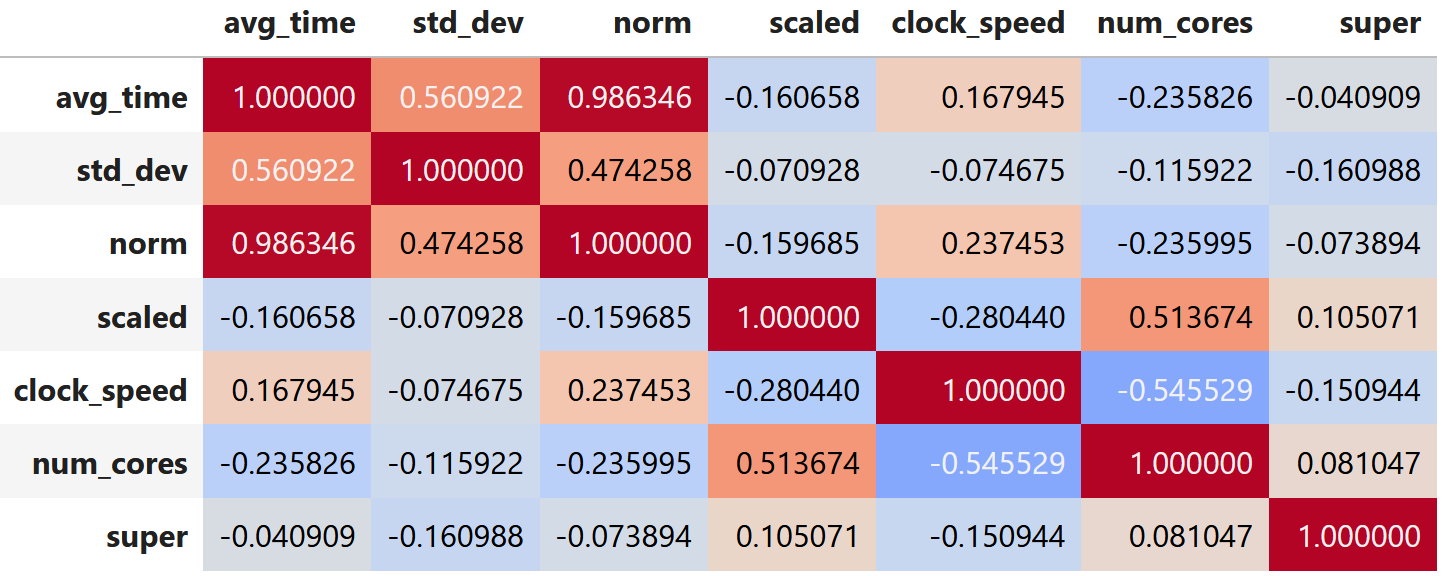
\includegraphics[width=\textwidth]{figures/final/xcorr_count_primes.png}
         \caption{``count\_primes"}
         \label{fig:normalized}
     \end{subfigure}
     \hfill
    \caption{ A cross correlation plot for the variables in our benchmarks using 4 processes. }
    \label{fig:xcorrelation}
\end{figure}


Finally, we observe the cross-correlation between the different variables in our experiments while using 4 processes, since this is the largest scale for the benchmarks that every computer ran. This is shown in Figure \ref{fig:xcorrelation}.
Unsurprisingly, for ``all\_to\_all", the direct times (avg\_time), normalized time (norm), and the scaled timings (scaled) are all correlated. Also unsurprisingly, the scaled times and number of cores are correlated, since we use the number of cores to calculate the scaled timings.

The same applies to ``count\_primes", however, the scaled timings are no longer correlated with the other timings. This may be because the direct timings span only three orders of magnitude, $10^{-4}$ to $10^{-1}$, whereas the results for ``all\_to\_all" span from $10^{-7}$ to $10^{-2}$, so the scaling with number of processors scales the timings into too tight of a range to be significant in the cross-correlation.

The cross-correlation plots also reveal a trend in the computers we selected for the experiments. The number of cores per node and the clock rate of the CPUs are negatively correlated, which suggests budgeting compromises while buying CPUs for a system.


\section{Conclusions}

In this project, we explored the notion that the computers found in HPC centers are significantly more powerful than commodity computers. We ran two benchmarks across commodity computers and single nodes of supercomputers: a low-compute and high-communication benchmark, and a low-network and high-compute benchmark.

We found that when running on a single-node, the supercomputers performed within the range of performance from commodity computers. The scale of the benchmarks was the most significant predictor of benchmark timings, while the clock speed showed almost no effect on the benchmark performance, all clock speeds falling within the range of 2.0 GHz to 3.6 GHz. For our benchmarks, this may not be a meaningful range of clock speeds.

Our results suggest that under our benchmarks, a single node on a supercomputer is not significantly different from a commodity computer.

\section{Future Work}
Future research goals will address complexities that were not covered in this project. A key area of focus will be on testing benchmarks that offer a more balanced mix of communication and computation, which will enable a more comprehensive understanding of how different computing architectures handle diverse workloads. Additionally, comparing processors with nearly identical specifications from various manufacturers, such as AMD, Intel, and IBM, will provide valuable insights into the subtleties of their performance characteristics. Another area of interest includes conducting tests to analyze communication speeds over the network, specifically by running benchmarks with one process per node. This approach will assess the efficiency of data transfer processes in different computing environments. Pursuing these areas of research will enhance and expand upon our current findings.
\printbibliography

\end{document}

%%%%%%%%%%%%%%%%%%%%%%%%%%%%%%%%%%%%%%%%%%%%%%%%%%%%%

\section{Current progress}
At the time of this report, we have written and run our all\_to\_all and count\_primes benchmarks on seven different machines. These machines are a combination of our personal computers and the CS machines at the University of New Mexico (UNM). We ran each benchmark using 1, 2, 4, 6, 8, 16, 32, 64, and 128 processes. For each run, we calculated the average and standard deviation of the amount of time to took to run one iteration of MPI\_Alltoall with a message size of 4196 bytes or one iteration of each process counting prime numbers between 0 and 10000 and performing a single MPI\_Allgather at the end. The GitHub repository for our project is included in our References section \cite{repo}. Preliminary results are included at the end of this report.

\section{Challenges}
We encountered unexpected difficulty running oversubscribed jobs on the CARC supercomputers. We have found a workaround to let us oversubscribe CARC nodes but creating this method delayed our results from CARC systems.

\section{Future Work}
The following work remains to be completed:
\begin{enumerate}
    \item Run our benchmarks on CARC systems.
    \item Analyze our results across the following metrics:
    \begin{enumerate}
        \item Plot average runtime versus number of processes.
        \item Compute and plot normalized time versus  number of processes. Normalized time will be calculated by multiplying average runtime by the clock speed of the processor.
        \item Compute and plot average runtime versus normalized cores. Normalized cores will be calculated by multiplying average runtime by number of cores available divided by the number of processes used.
        \item Plot normalized time by normalized cores.
    \end{enumerate}
    \begin{enumerate}
        \item These plots will indicate if network bandwidth is a limiting factor in our benchmarks or if there are other variables that effect runtime besides clock speed and number of cores on a processor.
    \end{enumerate}
    \item Formalize these findings in a written report.
\end{enumerate}

\section{Preliminary Results}

We ran the ``all\_to\_all" and ``count\_primes" benchmarks for each of the computers. Each benchmark repeats 1000 times consecutively, which we time and divide by 1000 to get the time for one benchmark iteration. We repeat this process 800 times. For Figures 1 through 4, each line corresponds to the mean across the 800 runs with the shaded area corresponding to one standard deviation either side of the mean. Figure \ref{fig:all_to_all} and Figure \ref{fig:count_primes} show the results of the benchmarks using the timings directly. 

For Figure \ref{fig:all_to_all_normalized} and Figure \ref{fig:count_primes_normalized}, we attempt to ``normalize" the results by multiplying each benchmark timing (seconds per benchmark) by the computer's clock speed (cycles per second) to get the timings in cycles per benchmark. 

In Figure \ref{fig:all_to_all_scaled} and Figure \ref{fig:count_primes_scaled}, we compare each computer's performance using a scaled metric - we multiply each benchmark time by the number of processes used and divide by the total number of cpu cores on the computer. 

Figure \ref{fig:correlation} shows the correlation between cpu clock speed and the seconds per benchmark across the different sizes of benchmark runs. Figure \ref{fig:xcorrelation} shows the cross correlation for different variables in the benchmark runs.

\begin{figure}[h]
    \centering
    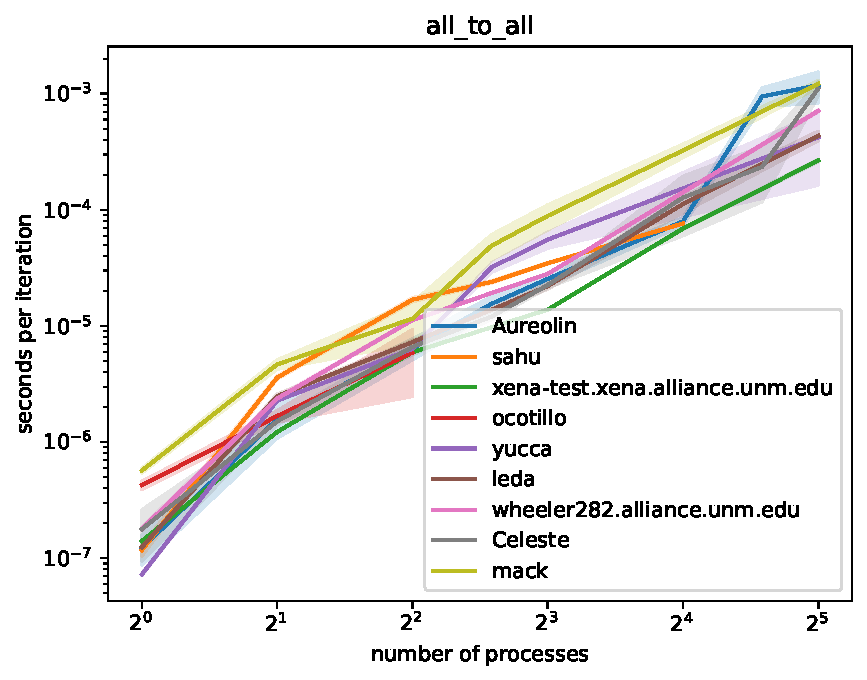
\includegraphics[width=0.8\textwidth]{figures/final/all_to_all.pdf}
    \caption{The results of the ``all\_to\_all" benchmarks across computers. Each line is the mean benchmark time across 800 repetitions with one standard deviation either side of the mean shaded in.}
    \label{fig:all_to_all}
\end{figure}

\begin{figure}[h]
    \centering
    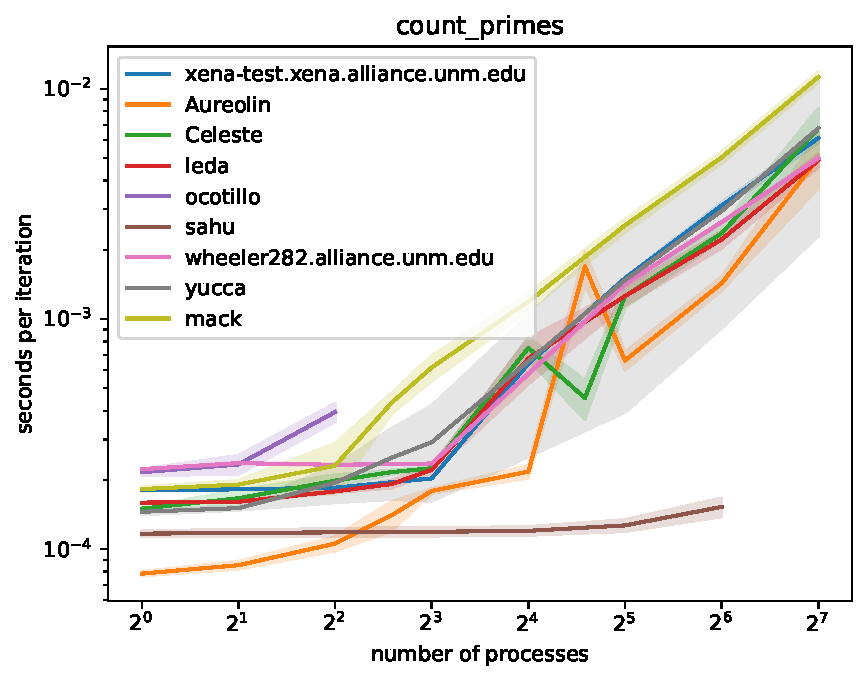
\includegraphics[width=0.8\textwidth]{figures/final/count_primes.pdf}
    \caption{The results of the ``count\_primes" benchmarks across computers. Each line is the mean benchmark time across 800 repetitions with one standard deviation either side of the mean shaded in.}
    \label{fig:count_primes}
\end{figure}

\begin{figure}[h]
    \centering
    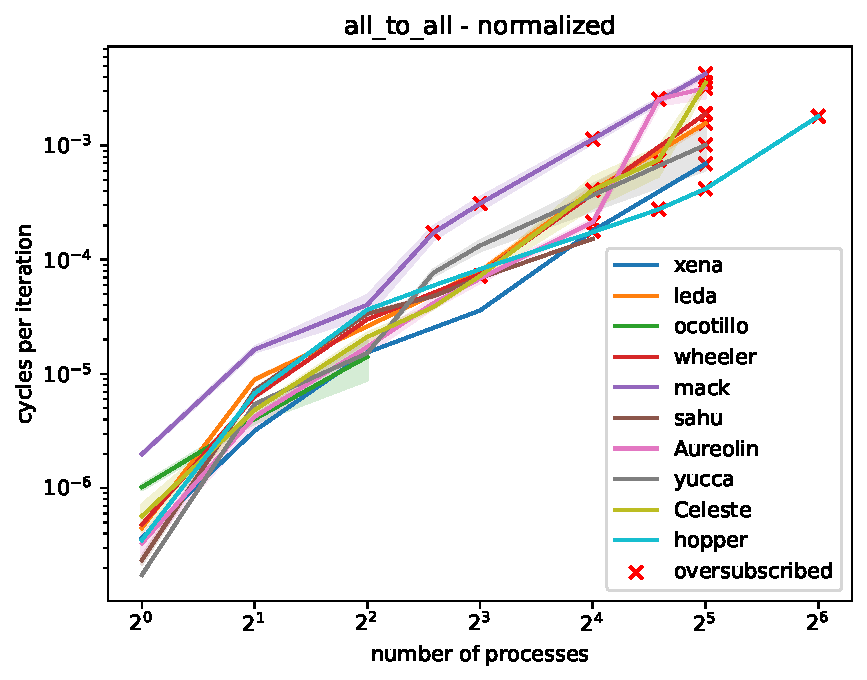
\includegraphics[width=0.8\textwidth]{figures/final/all_to_all_normalized.pdf}
    \caption{The results of the ``all\_to\_all" benchmarks across computers. Each line is the ``normalized" mean benchmark result in cycles per benchmark across 800 repetitions with one standard deviation either side of the mean shaded in. }
    \label{fig:all_to_all_normalized}
\end{figure}

\begin{figure}[h]
    \centering
    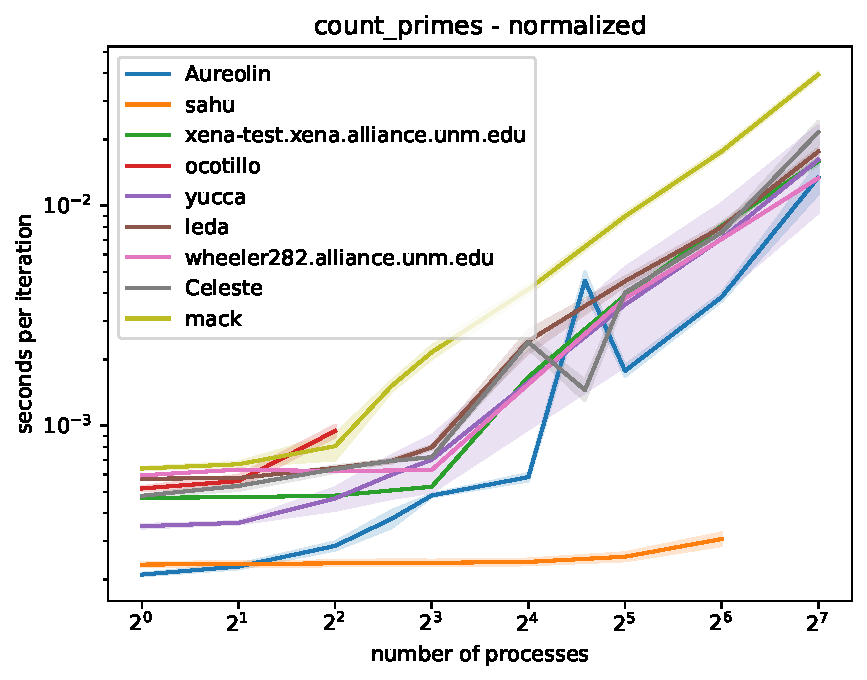
\includegraphics[width=0.8\textwidth]{figures/final/count_primes_normalized.pdf}
    \caption{The results of the ``count\_primes" benchmarks across computers. Each line is the ``normalized" mean benchmark result in cycles per benchmark across 800 repetitions with one standard deviation either side of the mean shaded in.}
    \label{fig:count_primes_normalized}
\end{figure}

\begin{figure}[h]
    \centering
    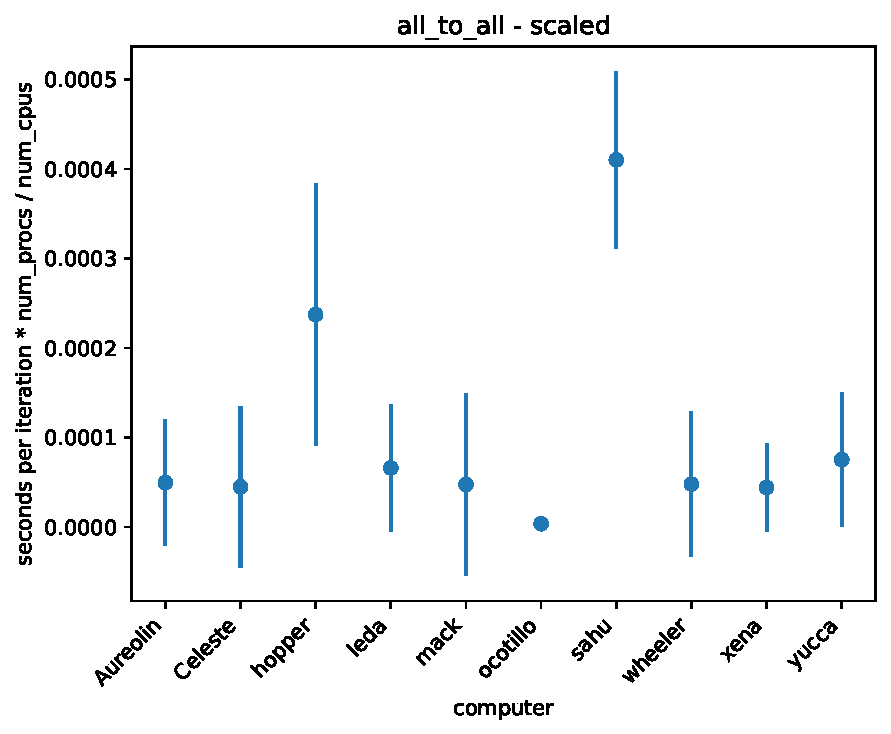
\includegraphics[width=0.8\textwidth]{figures/final/all_to_all_scaled.pdf}
    \caption{The scaled benchmark results for ``all\_to\_all" across computers.}
    \label{fig:all_to_all_scaled}
\end{figure}

\begin{figure}[h]
    \centering
    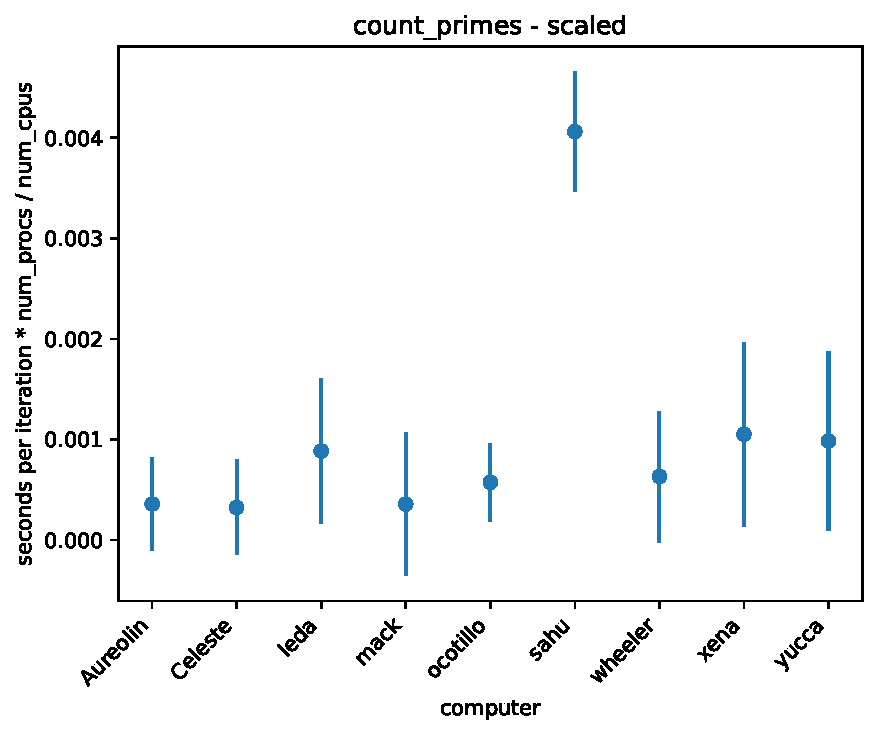
\includegraphics[width=0.8\textwidth]{figures/final/count_primes_scaled.pdf}
    \caption{The scaled benchmark results for ``count\_primes" across computers.}
    \label{fig:count_primes_scaled}
\end{figure}

\begin{figure}[h]
    \centering
    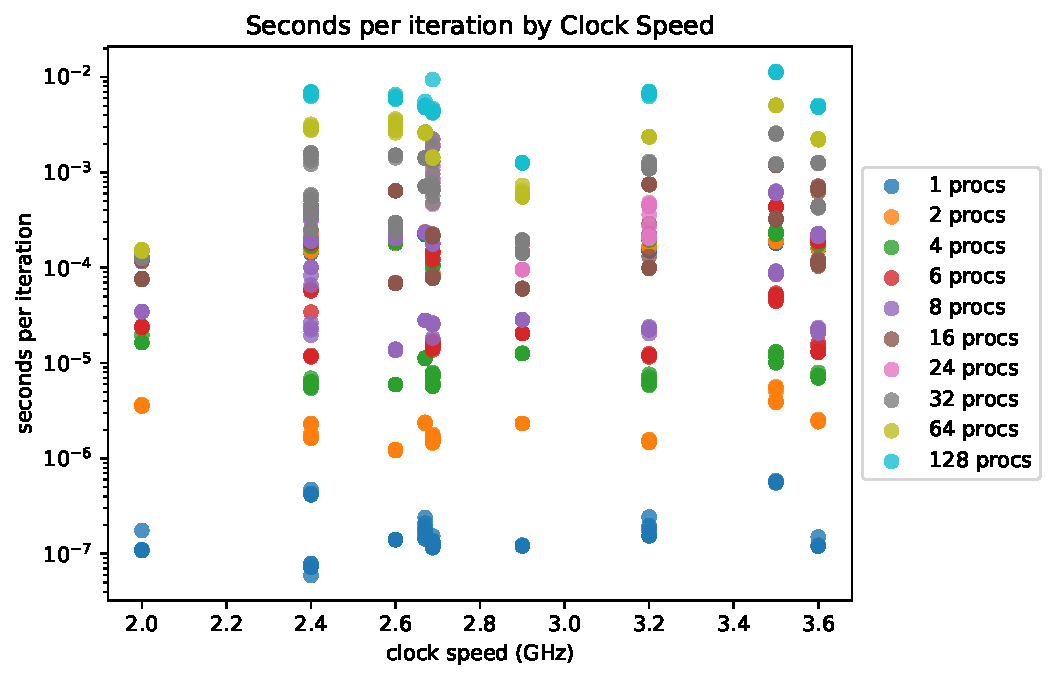
\includegraphics[width=0.8\textwidth]{figures/final/correlation.pdf}
    \caption{A correlation plot, showing the relationship between the clock speed of a cpu and how long each benchmark takes to run across the various sizes of benchmark. }
    \label{fig:correlation}
\end{figure}

\begin{figure}[h]
    \centering
    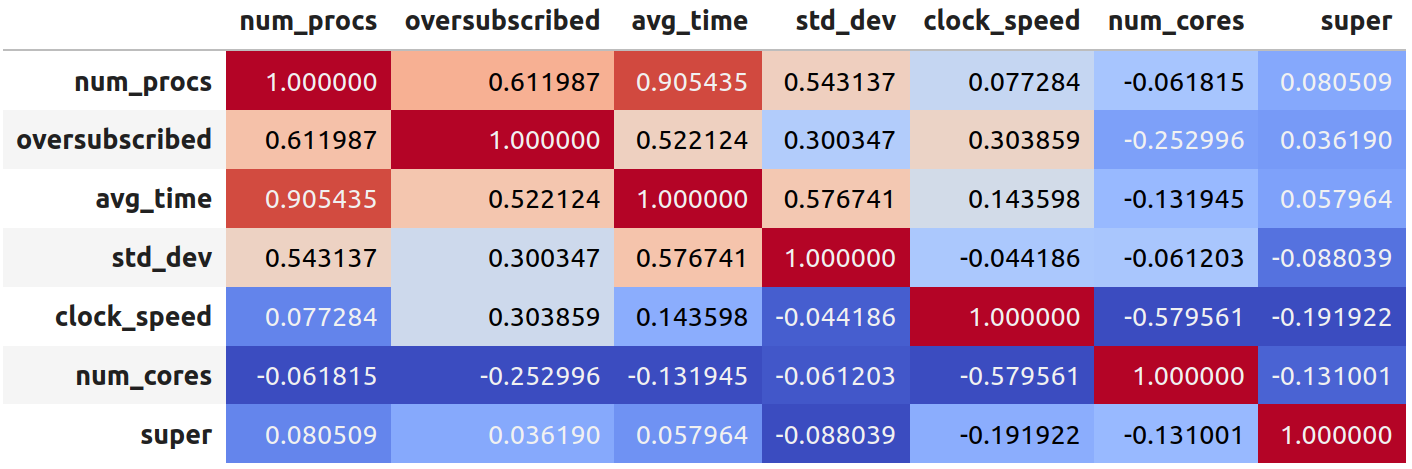
\includegraphics[width=0.8\textwidth]{figures/final/xcorr.png}
    \caption{A cross correlation plot for the variables in our benchmarks. }
    \label{fig:xcorrelation}
\end{figure}


Commands: \\
\textbf{lscpu} \\
if lspcu doesn't give clock speed, try \textbf{cat /proc/cpuinfo | grep Hz} \\

\begin{itemize}
\item Specs format: CPU model (Model name), Cores per node, Cores per socket, clock rate
    \item Hopper: Intel(R) Xeon(R) Gold 6226R, 64, 16, 2.90GHz
    \item Wheeler: Intel(R) Xeon(R) X5550, 8, 4, 2.67GHz
    \item Aureolin (Jason's laptop): 12th Gen Intel(R) Core(TM) i7-12700H, 10, 10, 2688 MHz
    \item Celeste (Jason's desktop): Intel(R) Core(TM) i7-8700, 6, 6, 3200 MHz
    \item Leda (CS machine): Intel(R) Core(TM) i9-9900K, 16, 8, 3.60GHz
    \item Trucks (CS machine): Intel(R) Xeon(R) CPU E5-2637 v4, 4, 1, 3.50GHz
    \item Sahu (TumorAI machine): Intel(R) Xeon(R) Gold 6338, 128, 32, 2.00GHz
    \item Xena: Intel(R) Xeon(R) CPU E5-2640 v3, 16, 8, 2.60GHz
    \item Ocotillo (Servilla's laptop): Intel(R) Core(TM) i7-5500U, 4, 2, 2.40GHz
    \item Yucca (Servilla'a Laptop): Intel(R) Core(TM) i9-10885H, 16, 8, 2.40GHz
\end{itemize}



\printbibliography

\end{document}


example cite: \cite{cfb_db}


\newpage
\nocite{*}
\bibliographystyle{acm}
\bibliography{references}
